% Exemplo: pôster (painel) de evento acadêmico, 90 x 120 cm, com a classe
% a0poster. É o mesmo pôster de poster-beamerposter.tex (feito com
% beamerposter), refeito com a a0poster: faixa com o nome do evento,
% título, autor e seções em duas colunas.
% Toda a arte (faixas, ondas, ícone) é desenhada com TikZ no fundo da
% página (pacote eso-pic) e as figuras são geradas no próprio documento:
% não há imagens de terceiros. As colunas são duas minipages; como figuras
% e tabelas flutuantes não funcionam dentro delas, as legendas são
% escritas com \captionof (caption).
% A a0poster só conhece os tamanhos A0 a A3: o painel de 90 x 120 cm é
% definido com o geometry (papersize), depois que a classe é carregada.
% Compilar: latexmk -pdf poster-a0poster.tex  (biber para as referências)
% Testado com: a0poster 1.22b, biblatex-abnt 3.4, TeX Live 2024 ou mais
% recente
%%BEGIN:aposterpreambulo
\documentclass[a0, portrait, final]{a0poster}
% A classe grava o tamanho A0 (83,96 x 118,82 cm) em
% \paperwidth/\paperheight e, no \begin{document}, em um
% \special{papersize} para o dvips. Para o painel de 90 x 120 cm: o
% geometry redefine o papel e as margens (e o tamanho do PDF), e
% \anullfalse desliga o \special da classe, que o pdflatex ignoraria com
% aviso.
\anullfalse
\usepackage[papersize={90cm,120cm}, left=6cm, right=6cm, top=19.1cm,
            bottom=5cm]{geometry}
\usepackage[T1]{fontenc}
\usepackage[brazilian]{babel}
% Latin Modern: fontes escaláveis para a matemática e o texto com serifa
% (a a0poster declara o Computer Modern OT1 só em alguns tamanhos, e a
% matemática sairia com tamanhos substituídos); depois vêm as fontes sem
% serifa e de máquina
\usepackage{lmodern}
% símbolos grandes (somatório) na escala do texto: o Latin Modern os declara
% com tamanho fixo de 10 pt
\DeclareFontFamily{OMX}{lmex}{}
\DeclareFontShape{OMX}{lmex}{m}{n}{<->lmex10}{}
\usepackage{helvet}              % sem serifa, com as medidas da Arial
\renewcommand{\familydefault}{\sfdefault}
\usepackage[varqu,varl,scaled=0.95]{inconsolata}  % fonte de máquina do livro
\usepackage{tikz}                % arte do painel, caixas e diagramas
\usetikzlibrary{positioning, calc}
\usepackage{pgfplots}            % gráfico de barras
\pgfplotsset{compat=1.18}
\usepackage{eso-pic}             % arte de fundo em todas as páginas
\usepackage{booktabs}
\usepackage{caption}             % \captionof: legendas fora de flutuantes
\usepackage{enumitem}            % listas com recuo e espaçamento do pôster
\usepackage{xurl}                % endereços longos quebram em qualquer ponto
\usepackage{ragged2e}            % texto justificado (\justifying)
% \justifying não recua os parágrafos
\setlength{\JustifyingParindent}{0pt}
\usepackage{csquotes}
% noslsn: referências sem [S. l.] e [s. n.]
\usepackage[backend=biber, style=abnt, noslsn]{biblatex}
\addbibresource{poster-evento.bib}
% Referências: tamanho da letra, entrelinha e espaço entre uma referência
% e a seguinte. Para mudar a aparência da lista, altere só estes três
% valores.
% tamanho da letra (o texto do pôster tem 36 pt)
\newcommand{\refletra}{24pt}
% distância entre as linhas de uma mesma referência
\newcommand{\refentrelinha}{29pt}
% espaço entre as referências; a NBR 6023 pede uma linha em branco
% (\baselineskip), que num pôster ocupa muito espaço
\newcommand{\refespaco}{0pt}
% O biblatex compõe a lista com \bibfont (e não com o tamanho em vigor);
% o biblatex-abnt usa \normalfont no subtítulo, que aqui voltaria ao
% tamanho do texto: na lista, ele só tira o negrito e o itálico. O espaço
% entre as referências vai no início do documento, porque o estilo abnt o
% define (com a linha em branco) no fim do preâmbulo.
\renewcommand*{\bibfont}{\fontsize{\refletra}{\refentrelinha}\selectfont
  \renewcommand*{\normalfont}{\mdseries\upshape}}
\AtBeginDocument{\appto{\bibsetup}{\setlength{\bibitemsep}{\refespaco}}}
%%END:aposterpreambulo

%%BEGIN:aposterestilo
% Tamanhos de letra pedidos pelo evento: texto com 36 pt (legível a 1 m),
% títulos das seções com 40 pt, título do trabalho com 72 pt. A a0poster
% já redefine \normalsize (24,88 pt), \small etc.: aqui eles são trocados
% de novo.
\renewcommand{\normalsize}{\fontsize{36}{44}\selectfont}
\renewcommand{\small}{\fontsize{30}{36}\selectfont}
\renewcommand{\footnotesize}{\fontsize{24}{29}\selectfont}
\renewcommand{\large}{\fontsize{40}{48}\selectfont}
\renewcommand{\Large}{\fontsize{50}{60}\selectfont}
\renewcommand{\Huge}{\fontsize{72}{84}\selectfont}
\setlength{\parindent}{0pt}

% Cores do painel
\definecolor{eventoescuro}{HTML}{0B3C5D}
\definecolor{eventomedio}{HTML}{1D7A8C}
\definecolor{eventodestaque}{HTML}{E07A1F}
\definecolor{eventotexto}{HTML}{4A4A4A}

% Arte do painel, desenhada com TikZ no fundo da página (eso-pic, origem no
% canto de baixo à esquerda): faixa do alto com o nome do evento, ícone de
% livro aberto e círculos; ondas no pé. A margem de cima do geometry (top)
% é a distância do alto da página até o título do trabalho.
\newcommand{\nomeevento}{SIMPÓSIO DE EXEMPLO 2026}
\newcommand{\lemaevento}{Ensino, pesquisa e extensão}
\AddToShipoutPictureBG{\put(0,0){%
  \begin{tikzpicture}[x=1cm, y=1cm]
    \useasboundingbox (0,0) rectangle (90,120);
    % faixa do alto, com a borda de baixo em onda
    \shade[left color=eventoescuro, right color=eventomedio]
      (0,120) -- (90,120) -- (90,106.5)
      .. controls (65,102.5) and (35,109) .. (0,104.5) -- cycle;
    % círculos translúcidos
    \foreach \x/\y/\r in {80/114/9, 69/119/5, 86/104/4, 8/118/4, 58/108/2.5}
      \fill[white, opacity=.07] (\x,\y) circle (\r);
    % ícone: livro aberto
    \begin{scope}[shift={(13.5,112.3)}, line width=4pt, white]
      \draw[fill=white, fill opacity=.15] (0,0)
        .. controls (-2.5,1) and (-5,1) .. (-7,0.2)
        -- (-7,-6.8) .. controls (-5,-6) and (-2.5,-6) .. (0,-7) -- cycle;
      \draw[fill=white, fill opacity=.15] (0,0)
        .. controls (2.5,1) and (5,1) .. (7,0.2)
        -- (7,-6.8) .. controls (5,-6) and (2.5,-6) .. (0,-7) -- cycle;
      \foreach \k in {1,2,3} {
        \draw[line width=2.5pt] (-5.8,-1.2*\k)
          .. controls (-4,-1.2*\k+.4) .. (-1.2,-1.2*\k-.2);
        \draw[line width=2.5pt] (5.8,-1.2*\k)
          .. controls (4,-1.2*\k+.4) .. (1.2,-1.2*\k-.2);
      }
    \end{scope}
    \node[anchor=west, text=white, font=\fontsize{80}{90}\selectfont\bfseries]
      at (25,113.2) {\nomeevento};
    \node[anchor=west, text=white, font=\fontsize{40}{48}\selectfont]
      at (25.3,108.6) {\lemaevento};
    % fio de destaque abaixo da faixa
    \draw[eventodestaque, line width=6pt] (6,101.5) -- (84,101.5);
    % ondas do pé
    \fill[eventomedio, opacity=.85] (0,0) -- (0,4.5)
      .. controls (25,8.5) and (55,1) .. (90,5.5) -- (90,0) -- cycle;
    \fill[eventodestaque, opacity=.9] (0,0) -- (0,2.2)
      .. controls (30,0.2) and (60,5.5) .. (90,2.5) -- (90,0) -- cycle;
  \end{tikzpicture}}}

% \secao{título}: caixa arredondada com contorno na cor do evento; o texto
% que segue é justificado, com hifenização
\newcommand{\secao}[1]{%
  \par\vspace{.9cm}\noindent
  \tikz\node[draw=eventomedio, line width=2.25pt, rounded corners=.65cm,
    minimum width=\linewidth-2.25pt, minimum height=3.3cm, align=center,
    text=eventoescuro, font=\large\bfseries]{\MakeUppercase{#1}};
  \par\vspace{.7cm}\justifying}

% Legendas numeradas acima da figura e da tabela (como pede a ABNT), com
% espaço para o texto antes e depois; \fonte escreve a fonte abaixo. O
% ambiente ilustracao centraliza o conteúdo (sem flutuar)
% (position=top: a legenda vem antes também nas figuras; sem isso, o caption
% põe o espaço skip acima da legenda de \captionof{figure})
% (color: o caption volta à cor padrão, preta, com \normalcolor)
\captionsetup{font={small, color=eventotexto}, labelfont=bf, labelsep=colon,
  skip=0pt, position=top, justification=centering}
\newenvironment{ilustracao}{\par\vspace{.8cm}\centering}{\par}
\newcommand{\fonte}[1]{\par\vspace{.4cm}{\small Fonte: #1\par}\vspace{1cm}}
% listas com o marcador laranja e o texto justificado
\setlist[itemize]{label=\textcolor{eventodestaque}{\textbullet},
  leftmargin=1.5cm, labelsep=.4cm, topsep=0pt, itemsep=0pt, parsep=0pt,
  before=\justifying}
% \cmd{nome}: comando do LaTeX destacado no código da Figura 2
\newcommand{\cmd}[1]{\textcolor{eventomedio}{\bfseries\textbackslash #1}}
% \marca{n}: marcador numerado, como os do livro (círculo laranja)
\newcommand{\marca}[1]{\tikz[baseline=(m.base)]\node[circle,
  fill=eventodestaque, text=white, inner sep=.12cm, font=\small\bfseries]
  (m) {#1};}
%%END:aposterestilo

%%BEGIN:aposterdados
% título em duas linhas (72 pt): \\ marca onde a linha quebra
\newcommand{\titulo}{LaTeX para documentos acadêmicos:\\ um livro e um guia
  aberto de exemplos testados}
\newcommand{\autor}{Rodrigo Smarzaro}
\newcommand{\instituicao}{Departamento de Exemplo, Universidade Exemplo
  (autor@exemplo.edu.br)}
% Apoio financeiro, centralizado no pé em coluna única: troque as imagens
% de exemplo (pacote mwe) pelos logotipos dos financiadores; \apoiofalse
% retira a seção
\newif\ifapoio
\apoiotrue
\newcommand{\apoiofinanceiro}{%
  \par\vspace{-.8cm}
  \begin{center}
  \begin{minipage}[t]{.45\linewidth}
    \secao{Apoio financeiro}
    \centering
    \includegraphics[height=3cm]{example-image-a}\hspace{2cm}%
    \includegraphics[height=3cm]{example-image-b}\hspace{2cm}%
    \includegraphics[height=3cm]{example-image-c}
  \end{minipage}
  \end{center}}
%%END:aposterdados

\begin{document}
\color{eventotexto}
%%BEGIN:apostertitulo
\begin{center}
  {\Huge\bfseries\color{eventoescuro}\titulo\par}
  \vspace{1.5cm}
  {\large\autor\par\instituicao\par}
\end{center}
%%END:apostertitulo

%%BEGIN:apostercolunas
% duas colunas em minipages alinhadas pelo alto
\noindent
\begin{minipage}[t]{.47\linewidth}
  \secao{Introdução}
    Trabalhos acadêmicos seguem normas detalhadas de formatação. O \LaTeX,
    criado por Lamport sobre o \TeX\ de Knuth, separa o conteúdo da forma:
    o autor escreve o texto e marca a estrutura, e o programa cuida da
    numeração, das referências cruzadas, das citações e da lista de
    referências \parencite{Lamport1994}. Mesmo assim, quem começa encontra
    material em português disperso, muitas vezes desatualizado, e exemplos
    que não compilam mais.

  \secao{Objetivos}
    \begin{itemize}
      \item Oferecer um livro em português sobre \LaTeX\ para trabalhos
        acadêmicos, artigos, apresentações e material didático.
      \item Manter um guia público, com licença aberta, em que todos os
        exemplos do livro compilam \parencite{latexacademico}.
      \item Mostrar o uso das normas da ABNT do início ao fim.
    \end{itemize}

  \secao{Metodologia}
    Cada exemplo nasce no guia e é compilado por testes automáticos a cada
    versão, com o \TeX\ Live mais recente. O livro não copia o código:
    inclui o trecho do próprio arquivo do guia, delimitado por marcadores, e
    a figura do resultado gerada a partir dele (Figura~\ref{fig:fluxo}).
    \begin{ilustracao}
      \captionof{figure}{Do guia público ao livro}\label{fig:fluxo}
      \begin{tikzpicture}[caixa/.style={draw=eventomedio, line width=2pt,
          rounded corners=.5cm, minimum width=13cm, minimum height=4.5cm,
          align=center}]
        \node[caixa] (guia) {\textbf{Guia público}\\exemplos testados};
        \node[caixa, right=7cm of guia] (livro) {\textbf{Livro}\\texto e
          figuras};
        \draw[-latex, line width=4pt, eventodestaque] (guia) -- (livro)
          node[midway, above=.3cm, font=\small] {trechos e}
          node[midway, below=.3cm, font=\small] {resultados};
      \end{tikzpicture}
      \fonte{elaborado pelo autor.}
    \end{ilustracao}
    \justifying
    No livro, cada exemplo forma uma unidade com o código e o resultado lado
    a lado, e marcadores numerados ligam o texto às linhas do código: a
    seção \marca{1} é numerada sozinha, e a fórmula \marca{2} sai em
    destaque, centralizada (Figura~\ref{fig:unidade}).
    \begin{ilustracao}
      \captionof{figure}{Uma unidade Exemplo: código e resultado}%
      \label{fig:unidade}
      \begin{minipage}[c]{.56\linewidth}
        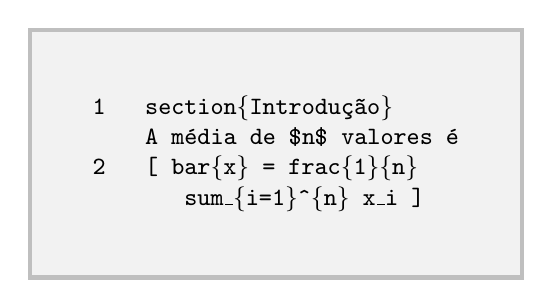
\begin{tikzpicture}
          \node[fill=black!5, draw=black!25, line width=1.5pt, inner sep=.8cm,
                font=\ttfamily\small, align=left] {%
            \begin{tabular}{@{}r@{\hspace{.5cm}}l@{}}
              \smash{\marca{1}} & \cmd{section}\{Introdução\} \\
                                & A média de \$n\$ valores é \\
              \smash{\marca{2}} & \cmd{[} \cmd{bar}\{x\} =
                                  \cmd{frac}\{1\}\{n\} \\
                                & \hspace*{1.5em}\cmd{sum}\_\{i=1\}%
                                  \textasciicircum\{n\} x\_i \cmd{]}
            \end{tabular}};
        \end{tikzpicture}
      \end{minipage}\hfill
      \begin{minipage}[c]{.4\linewidth}
        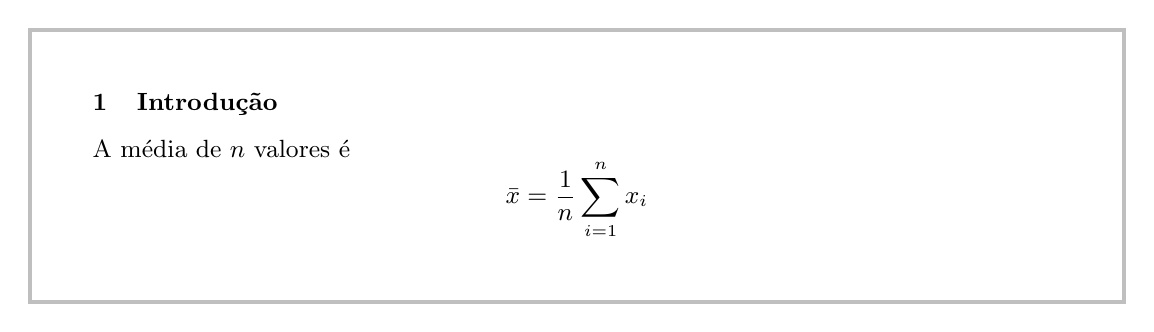
\begin{tikzpicture}
          \node[fill=white, draw=black!25, line width=1.5pt, inner sep=.8cm,
                align=left, text width=12.3cm, font=\rmfamily\small] {%
            {\bfseries 1\quad Introdução}\par\medskip
            A média de $n$ valores é
            \[ \bar{x} = \frac{1}{n}\sum_{i=1}^{n} x_i \]};
        \end{tikzpicture}
      \end{minipage}
      \fonte{elaborado pelo autor.}
    \end{ilustracao}
\end{minipage}\hfill
\begin{minipage}[t]{.47\linewidth}
  \secao{Resultados}
    O livro e o guia cobrem os principais tipos de documento acadêmico
    (Tabela~\ref{tab:numeros}), e os exemplos de trabalhos acadêmicos
    seguem a NBR 14724 \parencite{NBR14724}, com a classe abnTeX2
    \parencite{abntex2}. A Figura~\ref{fig:temas} mostra os temas com mais
    arquivos de exemplo no guia.
    \par\vspace{1.2cm}\noindent
    \begin{minipage}[t]{.46\linewidth}
      \centering
      \captionof{table}{Livro e guia em números}\label{tab:numeros}
      \begin{tabular}{@{}lr@{}}
        \toprule
        \textbf{Item}          & \textbf{Total} \\
        \midrule
        Capítulos              & 17 \\
        Apêndices              & 4 \\
        Exemplos comentados    & 81 \\
        Trechos de código      & 164 \\
        Exemplos no guia       & 88 \\
        Receitas no guia       & 81 \\
        \bottomrule
      \end{tabular}
      \fonte{elaborado pelo autor.}
    \end{minipage}\hfill
    \begin{minipage}[t]{.52\linewidth}
      \centering
      \captionof{figure}{Exemplos por tema no guia}\label{fig:temas}
      \begin{tikzpicture}
        \begin{axis}[xbar, width=12cm, height=15.5cm, xmin=0, xmax=12,
            bar width=.9cm, symbolic y coords={Áreas, Figuras, Tabelas,
              Apresentações, Diversão, Referências, Básico, Código},
            ytick=data, axis x line=none, axis y line*=left,
            nodes near coords, every node near coord/.style={font=\small},
            % números na fonte do texto (sem $...$, que usaria a fonte
            % da matemática)
            /pgf/number format/assume math mode,
            tick label style={font=\small}]
          \addplot[fill=eventomedio!75, draw=none] coordinates {(5,Áreas)
            (6,Figuras) (6,Tabelas) (8,Apresentações) (8,Diversão)
            (8,Referências) (10,Básico) (10,Código)};
        \end{axis}
      \end{tikzpicture}
      \fonte{elaborado pelo autor.}
    \end{minipage}

  \secao{Conclusões}
    Com os exemplos testados a cada versão, o código do livro continua
    compilando quando os pacotes mudam \parencite{Mittelbach2023}. O guia
    está aberto a pedidos de exemplos e correções, e o leitor encontra nele
    o arquivo completo de cada exemplo, pronto para compilar.

  % referências no fim da segunda coluna (só o apoio financeiro ocupa a
  % largura toda)
  \secao{Referências}
    \printbibliography[heading=none]
\end{minipage}
%%END:apostercolunas

%%BEGIN:aposterapoio
\ifapoio\apoiofinanceiro\fi
%%END:aposterapoio

\end{document}
